
\begin{frame}[t,allowframebreaks]{Gradient-based optimization -}


    \gls{ml}

    \framebreak

    %
    %

    Suppose $y=f(x)$ is a function whose domain and range is $\mathbb{R}$.\\
    \vspace{0.2cm}

    The \index{derivative}\gls{derivative} of $f(x)$, is another function 
    denoted as $f^\prime(x)$ or $df(x)/dx$.\\
    \vspace{0.2cm}
    
    The function $f^\prime(x)$:
    \begin{itemize}
        \item
        gives the {\bf slope of $f(x)$ at $x$} or, in other words,
        \item
        describes how to         
        scale a small change in the input $x$
        to compute a first-order approximation of the function $f$ at the new point:
        \begin{equation}
          f(x+\epsilon) \approx f(x) + \epsilon \; f^\prime(x)  
          \label{eq:deriv_1}
       \end{equation}\\
    \end{itemize}

    The \gls{derivative} $f^\prime(x)$ is useful for the 
    \index{extremization}\gls{extremization} of a function $f(x)$:\\
    It specifies how to make a small step in the space of $x$, 
    in order to make a small improvement in $f(x)$ in the desired direction.\\
    \vspace{0.2cm}

    The technique is known as \index{gradient descent}\gls{gradient descent},
    (often attributed to L.A. Cauchy 
    \cite{Cauchy:GradientDescent}).

    Starting from a point $\vect{x}$, 
    the \index{gradient descent}\gls{gradient descent} method 
    proposes a new point $\vect{x}^\prime$ 
    on the path towards the function minimum:
    \begin{equation}
        \vect{x} \rightarrow \vect{x}^\prime = 
          \vect{x} - \alpha \nabla_{\vect{x}} f(\vect{x})
        \label{eq:grad_descent_1}
     \end{equation}\\

    \framebreak

    %
    %

    \begin{center}
        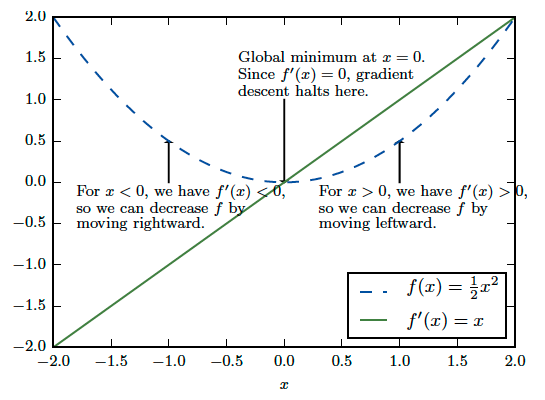
\includegraphics[width=0.75\textwidth]
            {./images/grad_descent/goodfellow17_grad_descent_1d.png}\\
        {\tiny 
            Simple illustration of the gradient descent technique.
            \color{col:attribution} 
            Schematic reproduced from p. 80 of \cite{Goodfellow:2017MITDL}.\\
        }
    \end{center}        

    \framebreak

    %
    %

    The \index{gradient descent}\gls{gradient descent} method
    readily generalizes in multiple dimensions.\\


    \begin{columns}
        \begin{column}{0.80\textwidth}
            \begin{center}
                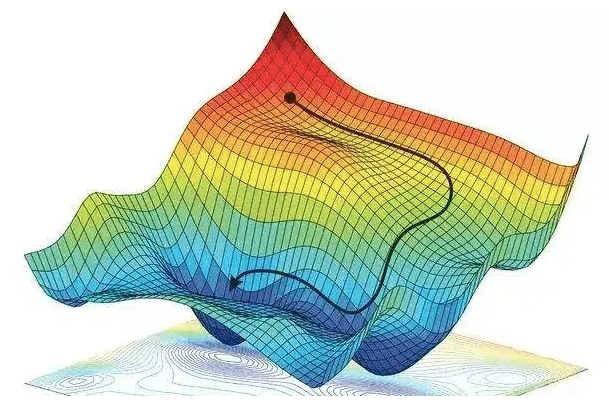
\includegraphics[width=0.99\textwidth]
                    {./images/grad_descent/guliyev20_grad_descent_2d.png}\\
                {\tiny 
                    Simple illustration of the gradient descent technique.
                    \color{col:attribution} 
                    Schematic reproduced from \cite{Medium:GradDescentOptLinReg}.\\
                }
            \end{center}                    
        \end{column}
        \begin{column}{0.20\textwidth}
        {\scriptsize
            The method has several weaknesses when applied to
            optimization problems in multiple dimensions.\\
            \vspace{0.2cm}
            Later in this lecture, 
            we will discuss these weaknesses and 
            improved algorithms.\\
        
        }    
        \end{column}
    \end{columns}

    \framebreak

    %
    %

    Points where the 
    \index{derivative}\gls{derivative} $f^\prime(x)$ 
    takes the value of 0  are known as 
    \index{critical point}\glspl{critical point} or 
    \index{stationary point}\glspl{stationary point}.\\

    \vspace{0.2cm}

    \begin{columns}
        \begin{column}{0.32\textwidth}
            These points are either: 
            \begin{itemize}
              \item \index{local minimum}\glspl{local minimum}, 
              \item \index{local maximum}\glspl{local maximum}, or
              \item \index{saddle point}\glspl{saddle point}.\\        
            \end{itemize}
            \end{column}
        \begin{column}{0.68\textwidth}

            \begin{center}
                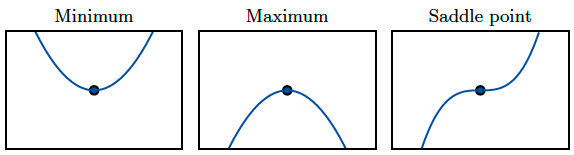
\includegraphics[width=0.80\textwidth]
                    {./images/grad_descent/goodfellow17_min_max_saddle_1d.png}\\
                {\tiny 
                    \color{col:attribution} 
                    Schematic reproduced from p. 81 of \cite{Goodfellow:2017MITDL}.\\
                }

                \vspace{0.6cm}

                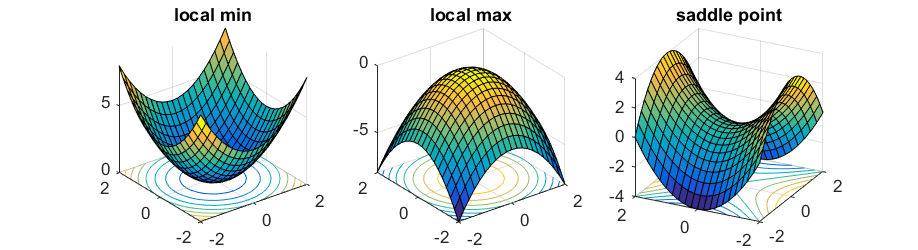
\includegraphics[width=0.99\textwidth]
                    {./images/grad_descent/ge16_min_max_saddle_2d.png}\\
                {\tiny 
                    \color{col:attribution} 
                    Schematic reproduced from \cite{OffConvex:EscapingSaddlePoints}.\\
                }
            \end{center}        
        
        \end{column}
    \end{columns}

\end{frame}


